\chapter{Introduction}
\section{Observation Networks}
\section{State of the Art}
\subsection{"Rules of Thumb for Sensor Placement"}
\subsection{Existing Metrics}
\subsection{Scale of Experiments}

\section{Requirements}
\subsection{Scope of Tool}
\subsection{Supported Workflows}
\subsection{Bathymetric File Support}
\subsection{Bathymetric Shadowing}
\subsection{Modeling Animal Movement and Habitat}
\paragraph{Ornstein-Uhlenbeck}
This is a paragraph about OU.
\paragraph{Random Walk}
\subsection{Evaluation of Sensor Emplacements}
\subsection{Selection of Optimal Emplacements}


Here is a picture in figure \ref{fig:example-1}.

\begin{figure}[htbp]
  \centering
  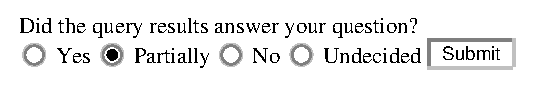
\includegraphics{example-figure.eps}
  \caption{An example of included Encapsulated PostScript (EPS).}
  \label{fig:example-1}
\end{figure}

In this modern age, you may find that you wish to include URLs or pathnames
which both tend to be long and hard for TeX to deal with because it doesn't
know where to insert linebreaks. The ``{\tt url}'' package (loaded in the main
uhtest.tex file) allows one to deal with these URLs. For example:

Here is an URL which cannot be broken, leading to terrible output
$<$http://www.hotwired.com/webmonkey/98/16/index2a.html$>$
%% The "<>" have to be entered in math mode, that's where the "$"s come from.

Using the package we get the much nicer \url{<http://www.hotwired.com/
webmonkey/98/16/index2a.html>} which LaTeX can handle just fine. Even better,
the parameter to {\tt $\backslash$url} can have spaces inserted anywhere so you
can make the LaTeX source lines in your text editor wrap nicely.

A few notes. It is recommended that you enclose your URLs in ``$<>$'' to ensure
that any punctuation around the URL won't be confused as part of the URL. You
can use URLs in your bibliography too (see the {\tt uhtest.bib} file for an
example). Finally, if you need to use a tilde in your URL then things are a
little trickier. One way to do it is like this:
\url{<http://www.dartmouth.edu/}$\sim$\url{jonh/ff-cache/1.html>}. The {\tt
$\backslash$url} style uses math mode internally, so we break the URL into two
pieces, and stick a tilde from math mode inbetween the two parts.

